\chapter{Experiments and Results}
\label{cha:experiments}

\section{Experimental Plan}
\label{sec:experimentalPlan}

\begin{comment}
Trying and failing is a major part of research. However, to have a chance of success you need a plan driving the experimental research, just as you need a plan for your literature search. Further, plans are made to be revised and this revision ensures that any further decisions made are in line with the work already completed.

The plan should include what experiments or series of experiments are planned and what questions the individual or set of experiments aim to answer. Such questions should be connected to your research questions, so that in the evaluation of your results you can discuss the results wrt to the research questions.
\end{comment}

In order to evaluate GeoGPT's ability to perform geospatial analyses, a Q\&A dataset was constructed. This dataset consists of geospatial questions with corresponding correct answers. For each sample of the dataset, a description of how a human would find it natural to approach the problem. This description is provided  as step-by-step path towards the solution, and is only included to guide any reader of this thesis as to how the system would be expected to solve the system. Only the questions and their answers are used in the actual evaluation. The full Q\&A dataset can be found in \autoref{app:qa-for-benchmark}.

Each question is labelled with a difficulty; one of \texttt{\{1, 2, 3\}}, with \texttt{3} being the most difficult. By having questions of varying difficulties, it will be easier to estimate the system's strength. There are X\todo{update} questions for each difficulty.

\section{Experimental Setup}
\label{sec:experimentalSetup}




\begin{comment}
The experimental setup should include all data --- parameters, etc. --- that would allow a person to repeat your experiments.
This will thus be the actual instantiation for each experiment of the general architecture described in Chapter~\ref{cha:architecture}.
\end{comment}
\section{Experimental Results}
\label{sec:experimentalResults}

\begin{comment}
Results should be clearly displayed and should provide a suitable representation of your results for the points you wish to make.
Graphs should be labelled in a legible font. If more than one result is displayed in the same graph, then these should be clearly marked.
Please choose carefully rather than presenting every result. Too much information is hard to read and often hides the key information you wish to present. Make use of statistical methods when presenting results, where possible to strengthen the results.
Further, the format of the presentation of results should be chosen based on what issues in the results you wish to highlight.
You may wish to present a subset in the experimental section and provide additional results in an appendix.
Point out specifics here but save the overall/general discussion to the Discussion chapter.
\end{comment}

\begin{figure}[htbp]
    \centering
    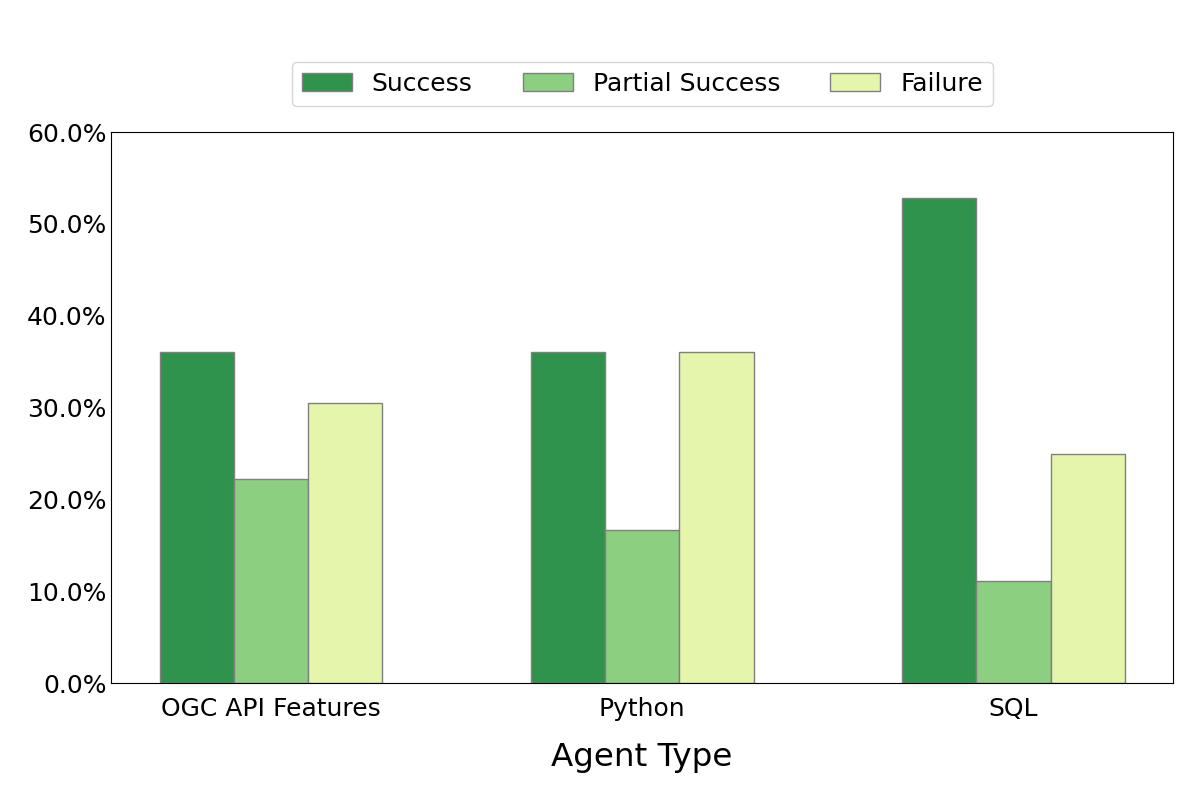
\includegraphics[width=\textwidth]{outcome_distribution_bar_chart.png}
    \caption{Outcome Distribution}
    \label{fig:outcome_distribution}
\end{figure}

\begin{figure}[htbp]
    \centering
    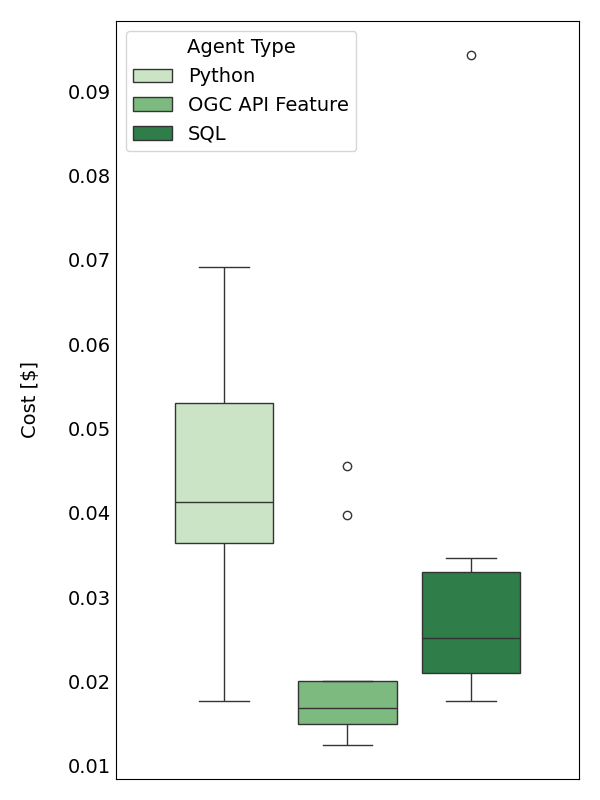
\includegraphics[width=0.8\textwidth]{cost_box_plot.png}
    \caption{Cost per Agent Type}
    \label{fig:cost_box_plot}
\end{figure}

\begin{figure}[htbp]
    \centering
    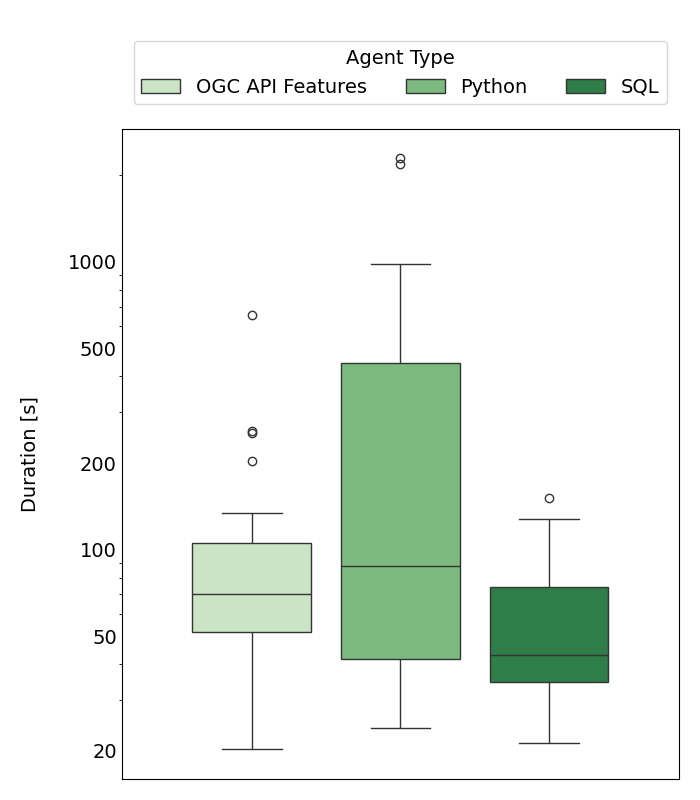
\includegraphics[width=0.8\textwidth]{duration_box_plot.png}
    \caption{Duration per Agent Type}
    \label{fig:duration_box_plot}
\end{figure}

